\chapter{Literary Review}
\label{chap:litrev}
\graphicspath{Chapter1/img/}


This chapter reviews the literature that informs the study of the policy--practice
gap in AI-in-education governance. It focuses on how AI policy is framed, how its
implementation is discussed, and how public sentiment helps reveal the conditions
under which AI adoption is accepted, questioned, or resisted in educational settings.

The review is organised around three connected areas. Section~\ref{c1:npf} examines
national policy and guidance documents from Ireland, France, Australia, and the
United States in order to identify how different governance systems define
AI-related priorities, risks, responsibilities, and expectations for implementation.
Section~\ref{c1:eps} reviews evidence on public sentiment and stakeholder
perspectives, with particular attention to European evidence as a cautious proxy for
wider Western trends. This part of the review considers how teachers, students,
parents, and the wider public perceive issues such as trust, fairness, ethical use,
teacher preparedness, access, and the social consequences of AI in education.
Section~\ref{c1:nlpsa} then reviews computational approaches to policy and sentiment
analysis, especially NLP methods such as topic modelling, sentiment analysis, and
selected elements of causal NLP, as well as the use of synthetic data to address gaps
and imbalance in available sentiment data.

By bringing these areas together, the chapter establishes the conceptual and
methodological basis for the study. It shows that AI governance, public sentiment,
and educational implementation are often examined separately, even though they are
closely connected in practice. The chapter therefore identifies the need for a
multi-layered, data-driven framework capable of linking policy language, stakeholder
discourse, sentiment evidence, and implementation challenges in the analysis of
AI-in-education governance.


\section{National Policy Frameworks}
\label{c1:npf}

As outlined in Chapter~\ref{chpt:intro}, Ireland, France, Australia, and the United
States were selected to provide a varied set of governance contexts for examining AI
education policy. This section develops that comparison by reviewing each national
framework in turn, with attention to how policy priorities, regulatory assumptions,
implementation responsibilities, and educational risks are framed.

The purpose of this review is not only to describe national policy positions, but to
identify how different governance settings shape the relationship between policy
intention and educational practice. The country-specific subsections that follow
therefore examine each case in relation to the wider policy--practice gap, focusing
on the extent to which guidance is made operational, responsibilities are clarified,
and implementation challenges are addressed.

\begin{figure}[ht]
    \centering
    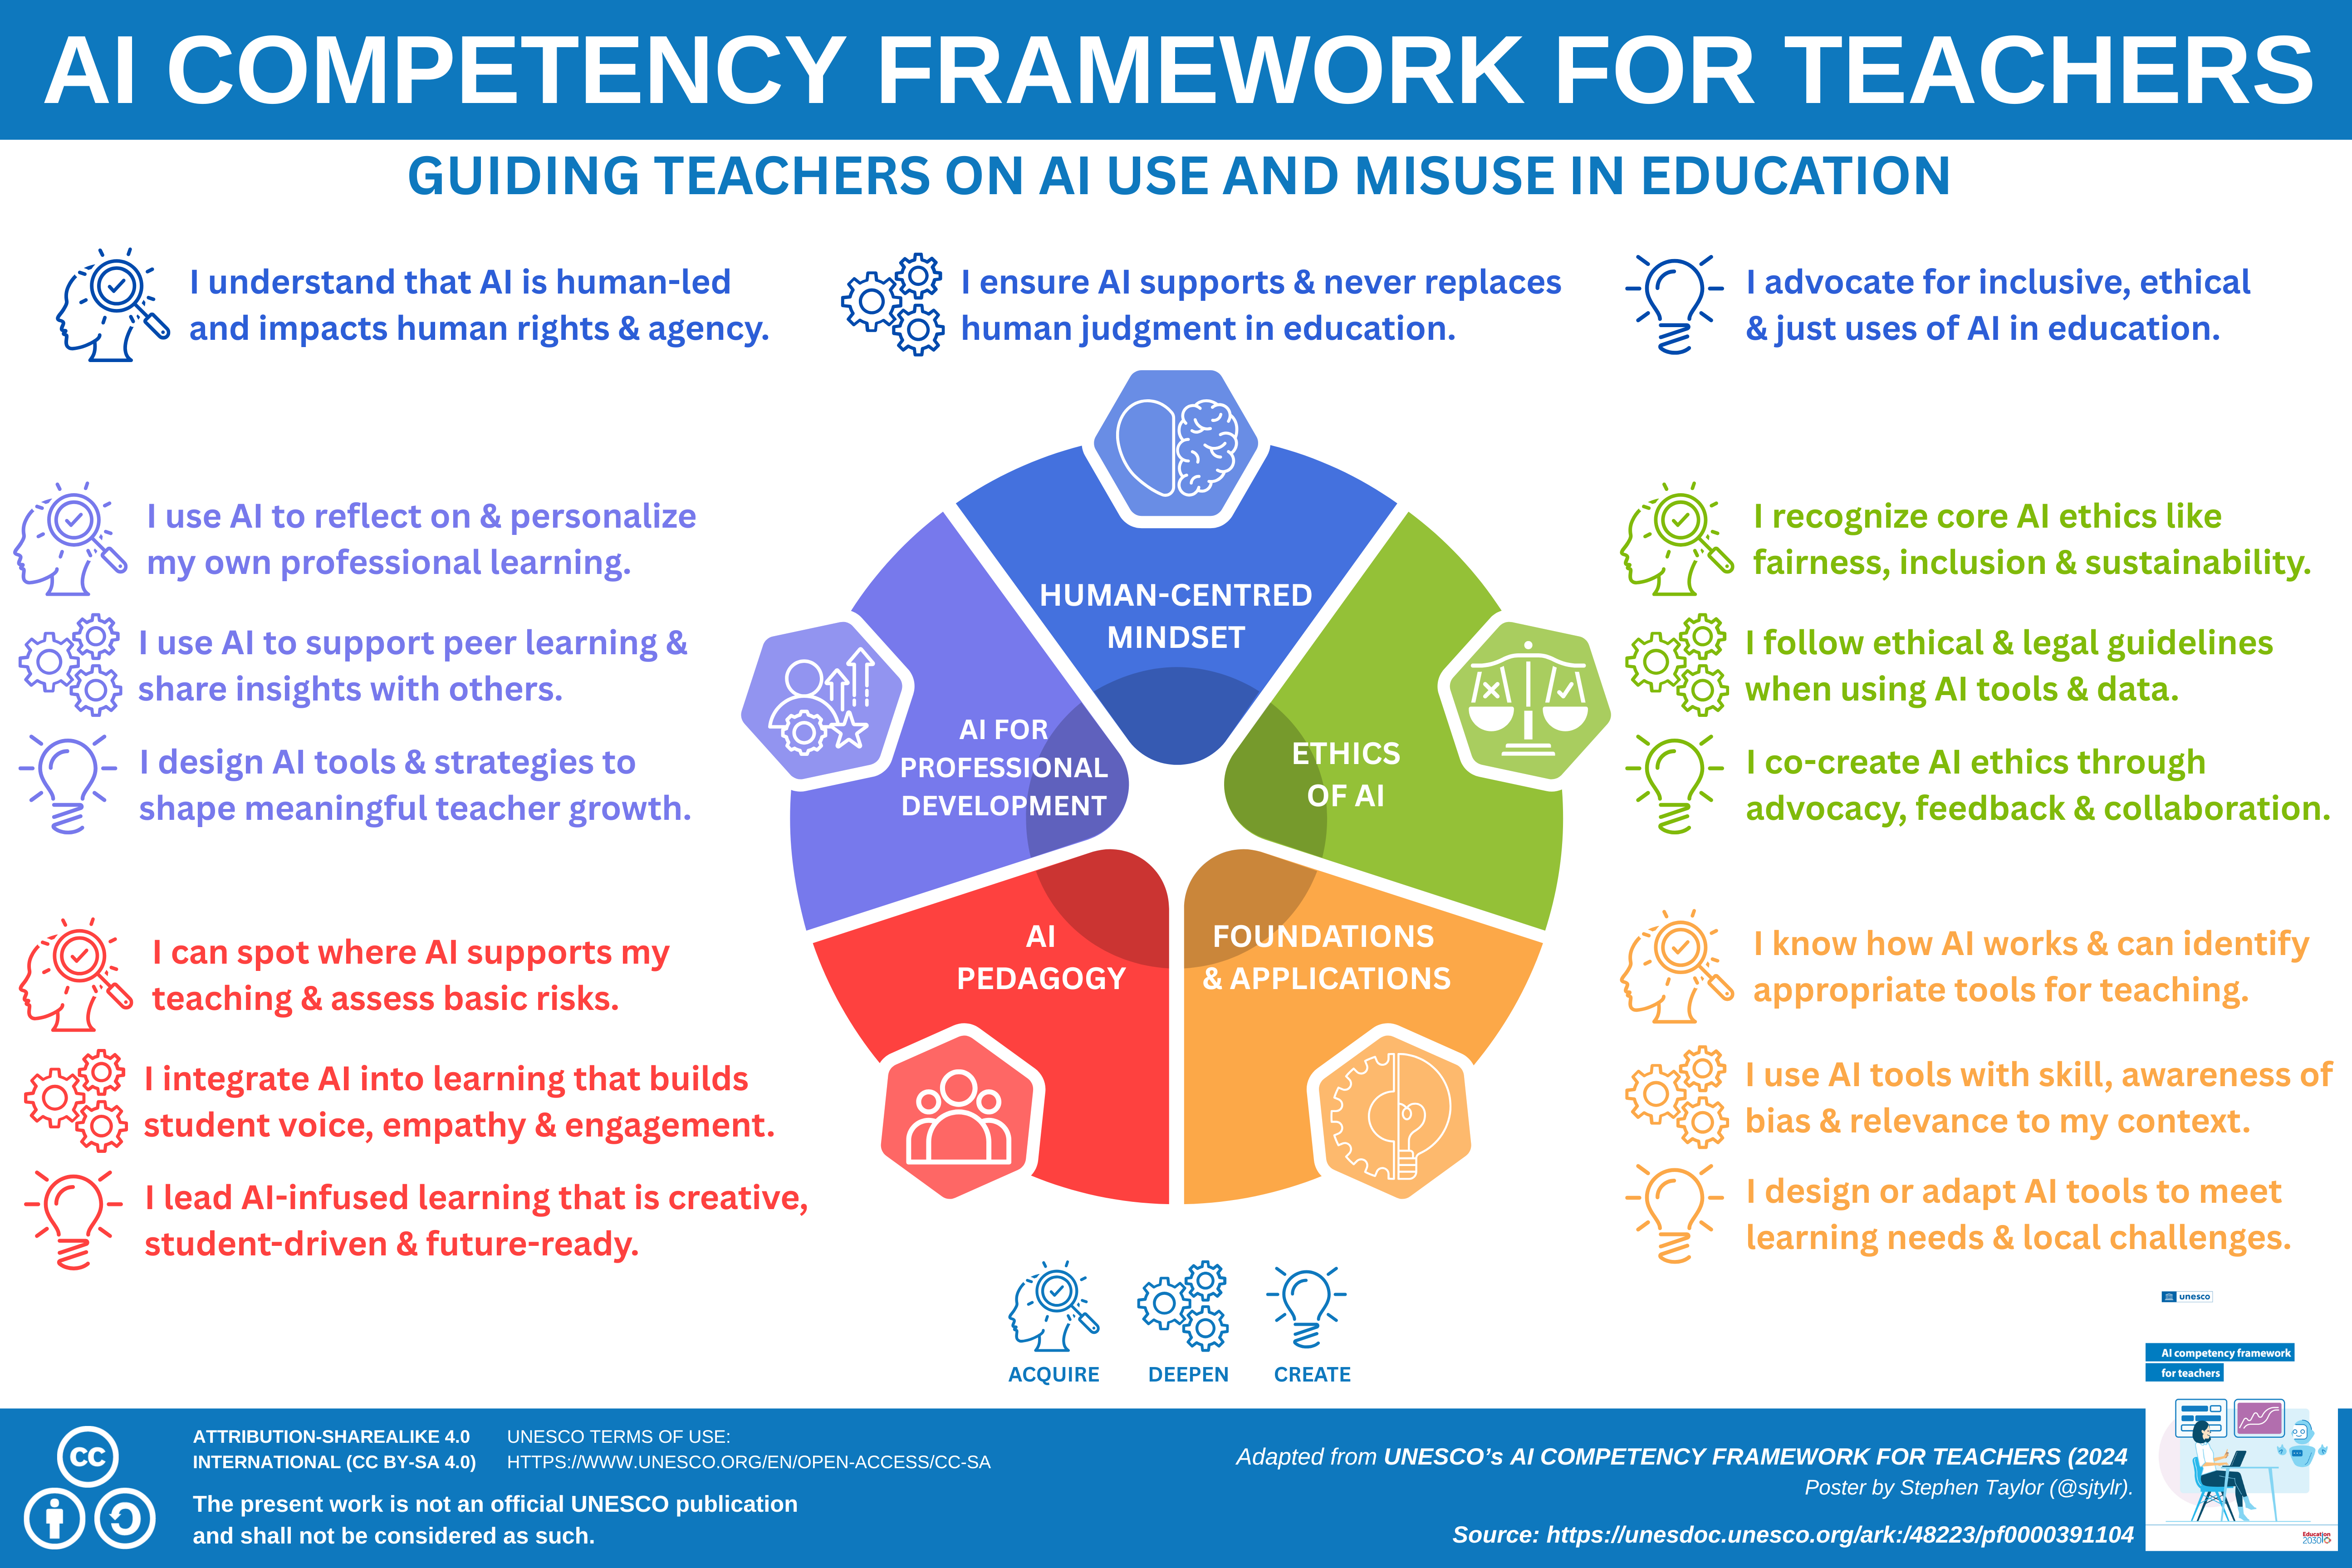
\includegraphics[scale=0.1]{Chapter1/img/unesco-ai-competencies-for-teachers-sjtylr.png}
    \caption{Overview of UNESCO's \textit{AI Competency Framework for Teachers}, whose emphasis on teacher capability, ethical awareness, pedagogical use, and professional learning is reflected in Ireland's emerging AI-in-education policy and guidance. Source: adapted from the framework by \cite{miao2024aiteachers}.}
    \label{fig:unesco-ai-competency-framework}
\end{figure}

\subsection{Ireland}

Ireland's approach to AI in education combines a high-level digital strategy with
emerging, sector-specific guidance responding to the rapid development of GenAI.
According to \cite{govie2025digitalstrategy}, the national agenda is framed by the
\textit{Digital Strategy for Schools to 2027}, which aims to support digital
transformation and strengthen digital competence among teachers and learners while
aligning Irish policy with wider European digital education priorities. As discussed
in Chapter~\ref{chpt:intro}, this direction is broadly consistent with the UNESCO
\textit{AI Competency Framework for Teachers} by \cite{miao2024aiteachers}, which
emphasises that AI integration depends not only on access to technology but also on
teacher capability, ethical awareness, pedagogical use and professional learning.
Figure~\ref{fig:unesco-ai-competency-framework} provides an overview of the
framework's main dimensions, covering a human-centred mindset, AI ethics, foundations
and applications, pedagogy and professional development. The 2024 Implementation Plan
by \cite{govie2025implementationplan} makes this agenda more operational by setting
actions for teacher professional learning, digital infrastructure, online safety,
digital leadership and AI-specific supports. It records important completed actions,
including an AI Hub for teachers and school leaders, digital leadership training,
digital communities of practice for DEIS schools supported through Ireland's
\textit{Delivering Equality of Opportunity in Schools} programme, and online safety
resources. At the same time, further work remains in progress on professional
learning, infrastructure guidance, procurement frameworks, cybersecurity, EU
engagement and AI-specific support for schools and classroom routines.

As set out by \cite{govie2025ainschools}, the \textit{Guidance on Artificial
Intelligence in Schools} builds on this wider strategy by offering more direct
support to teachers and school leaders. It sets out principles for safe, ethical, and
appropriate AI use, with attention to privacy, data protection, human oversight,
transparency, bias, and the need for teachers to verify AI-generated outputs. It also
points schools towards practical supports, including the AI in Schools Hub, an
introductory online course, and a 4P approach based on purpose, planning, policies,
and classroom practice.

However, the guidance also illustrates the limits of the current policy response. It
is presented as a first version and a living document, which suggests that many
aspects of implementation remain unsettled, especially assessment, monitoring,
teacher readiness, and the evaluation of AI's impact on learning. As set out by
\cite{aiadvisorycouncil2025aieducation}, the AI Advisory Council's \textit{AI and
Education Advice Paper} makes this point more explicitly, arguing that the rapid
uptake of GenAI has created uncertainty for teachers, students, and parents around
appropriate use, assessment, and academic integrity. The Council also warns that AI
detection tools are not a reliable solution, and calls instead for constructive use,
stronger AI literacy, clearer guidance, and regular policy updates. Its equity
concerns are also significant, particularly in relation to unequal access to paid AI
tools and the limited support for the Irish language, which may disadvantage
Gaelscoileanna.

In response to these uncertainties, local institutions and education bodies have
developed their own policies, focusing on ethical use, academic integrity, and
practical guidance for learners, as shown by \cite{stmarys2025aipolicy} and
\cite{cmetb2025guide}. This local response points to the limited availability of
fully practical national guidance and shows how schools are interpreting policy
within their own contexts. At a broader level, \cite{oecd2025ireland} similarly
stresses the need to evaluate how digital technologies affect student learning,
strengthen digital competence, and support equitable access, drawing on peer
experience from systems such as Estonia, France and Sweden.

Research from Irish institutions reinforces this mixed picture. \cite{byrne2024genai}
note that GenAI may support lesson preparation, personalised learning, feedback, and
administrative efficiency, while raising concerns about reliability, data privacy,
unequal access, academic integrity and responsible use. They further note that the
high cost of developing foundation models concentrates capacity among a few
providers, leaving many institutions dependent on external tools. Ongoing policy
development reflects this same tension. The \textit{First Interim Report}, presented by
\cite{jointcommittee2025interim}, calls for a coordinated national approach to AI
governance, stronger public and institutional AI literacy, effective implementation
of the EU AI Act discussed in \cite{eu2024aiact}, and safeguards for transparency,
equality, children's rights and equitable access.
Taken together, these developments illustrate a system in transition: strategic
ambition is clear, but implementation and oversight remain uneven, leaving a visible
policy--practice gap in guidance, teacher support and institutional responses to AI
in education.


\subsection{France}

France's approach to AI is shaped by a strong national ambition to reduce
technological dependence and position the country as a leading European actor in AI.
The report \textit{Our AI: Our Ambition for France} by
\cite{aicommission2024ambition} presents AI as both an economic opportunity and a
sovereignty challenge. It calls for investment in computing capacity, better data
access, research systems and training, alongside public-sector transformation that
remains human-centred, responsible and internationally governed. Within education,
this ambition provides the wider context for a more structured approach to AI
literacy, teacher support and regulation of AI use in schools.

This strategic ambition is accompanied by a regulatory approach shaped by both
European and national frameworks. As described by \cite{france2025aipolicy},
France's AI policy is closely linked to the EU AI Act, while also drawing on
domestic measures in areas such as data protection, intellectual property,
algorithmic transparency, and sector-specific oversight. Rather than developing a
single comprehensive national AI law, France appears to be adapting existing legal
and policy instruments to AI-related challenges. The French case therefore
illustrates a relatively coherent model in which EU regulation provides the main
legal structure, while national measures translate these principles into domestic
governance practice.

At the level of educational practice, \cite{menj2025cadreusage} introduced
\textit{L'IA en éducation : cadre d'usage}, a framework for the ethical, legal, and
pedagogical use of AI in schools. It authorises AI use only within defined
conditions, distinguishes between predictive and GenAI, warns against
non-sovereign public tools where personal or protected data are involved, and
stresses transparency, critical verification, and the adaptation of assessment
practices. This approach also aligns with UNESCO guidance on GenAI in education by
\cite{giannini2023generativeai}, which stresses critical, ethical, and pedagogical
teacher preparedness. National research from the \textit{Direction du Numérique pour
l'Éducation}, presented in \cite{dne2024intelligence}, further supports this
orientation by reviewing AI in education through public policy, ethics, classroom
applications, teacher training, and recent developments in GenAI. The report
highlights the need to develop critical thinking, data awareness, ethical judgement
and a basic understanding of AI systems, while ensuring that AI supports rather than
replaces teachers' professional role. Together, these elements suggest a deliberate
effort to embed AI in education through teacher development, ethical guidance and
structured pedagogical use. They also link AI literacy with assessment, data protection, and teacher agency.

Despite this structured policy environment, implementation challenges remain. The
report by \cite{igesr2025ia} states that AI use in schools is still uneven and often
shaped by individual teachers or local initiatives rather than a shared institutional
strategy. It identifies teacher training as a major weakness, calling for clearer
guidance, practical support and a large-scale national training effort. The report
also stresses stronger coordination across school, academic and national levels to
support consistent and equitable deployment in practice over time. Empirical evidence
from the AI4T project gives a more practical view of these training needs and
classroom adoption barriers. The French national evaluation by \cite{paris2023ai4t}
shows that targeted professional learning can strengthen teachers' understanding of
AI and support more informed classroom use. However, it also suggests that
participation and impact depend on access to training, institutional support,
teacher confidence and time for experimentation.

Overall, the French case shows a system that is comparatively well-structured at the
policy level, but still constrained by uneven implementation in practice. Its main
challenge is to translate national ambition and regulatory clarity into consistent
classroom-level capacity, while balancing pedagogical innovation with digital
citizenship, student development, and technological sovereignty.

\subsection{Australia}

The rapid rise of GenAI in late 2022 led to a swift and coordinated response across
Australian education. At the national level, this response is set out in the
\textit{Australian Framework for Generative Artificial Intelligence in Schools} by
\cite{dese2023australianframework}, developed with input from jurisdictions, school
sectors and national education agencies. The framework offers guidance for
policymakers, school leaders, teachers, support staff, parents and students. Its
principle-based design fits Australia's federal school system, where responsibilities
are shared across states, territories and sectors in practice and policy development.
Its six principles cover teaching and learning, wellbeing, openness, fairness,
accountability, privacy, security, safety, and responsible implementation.

\begin{figure}[ht]
    \centering
    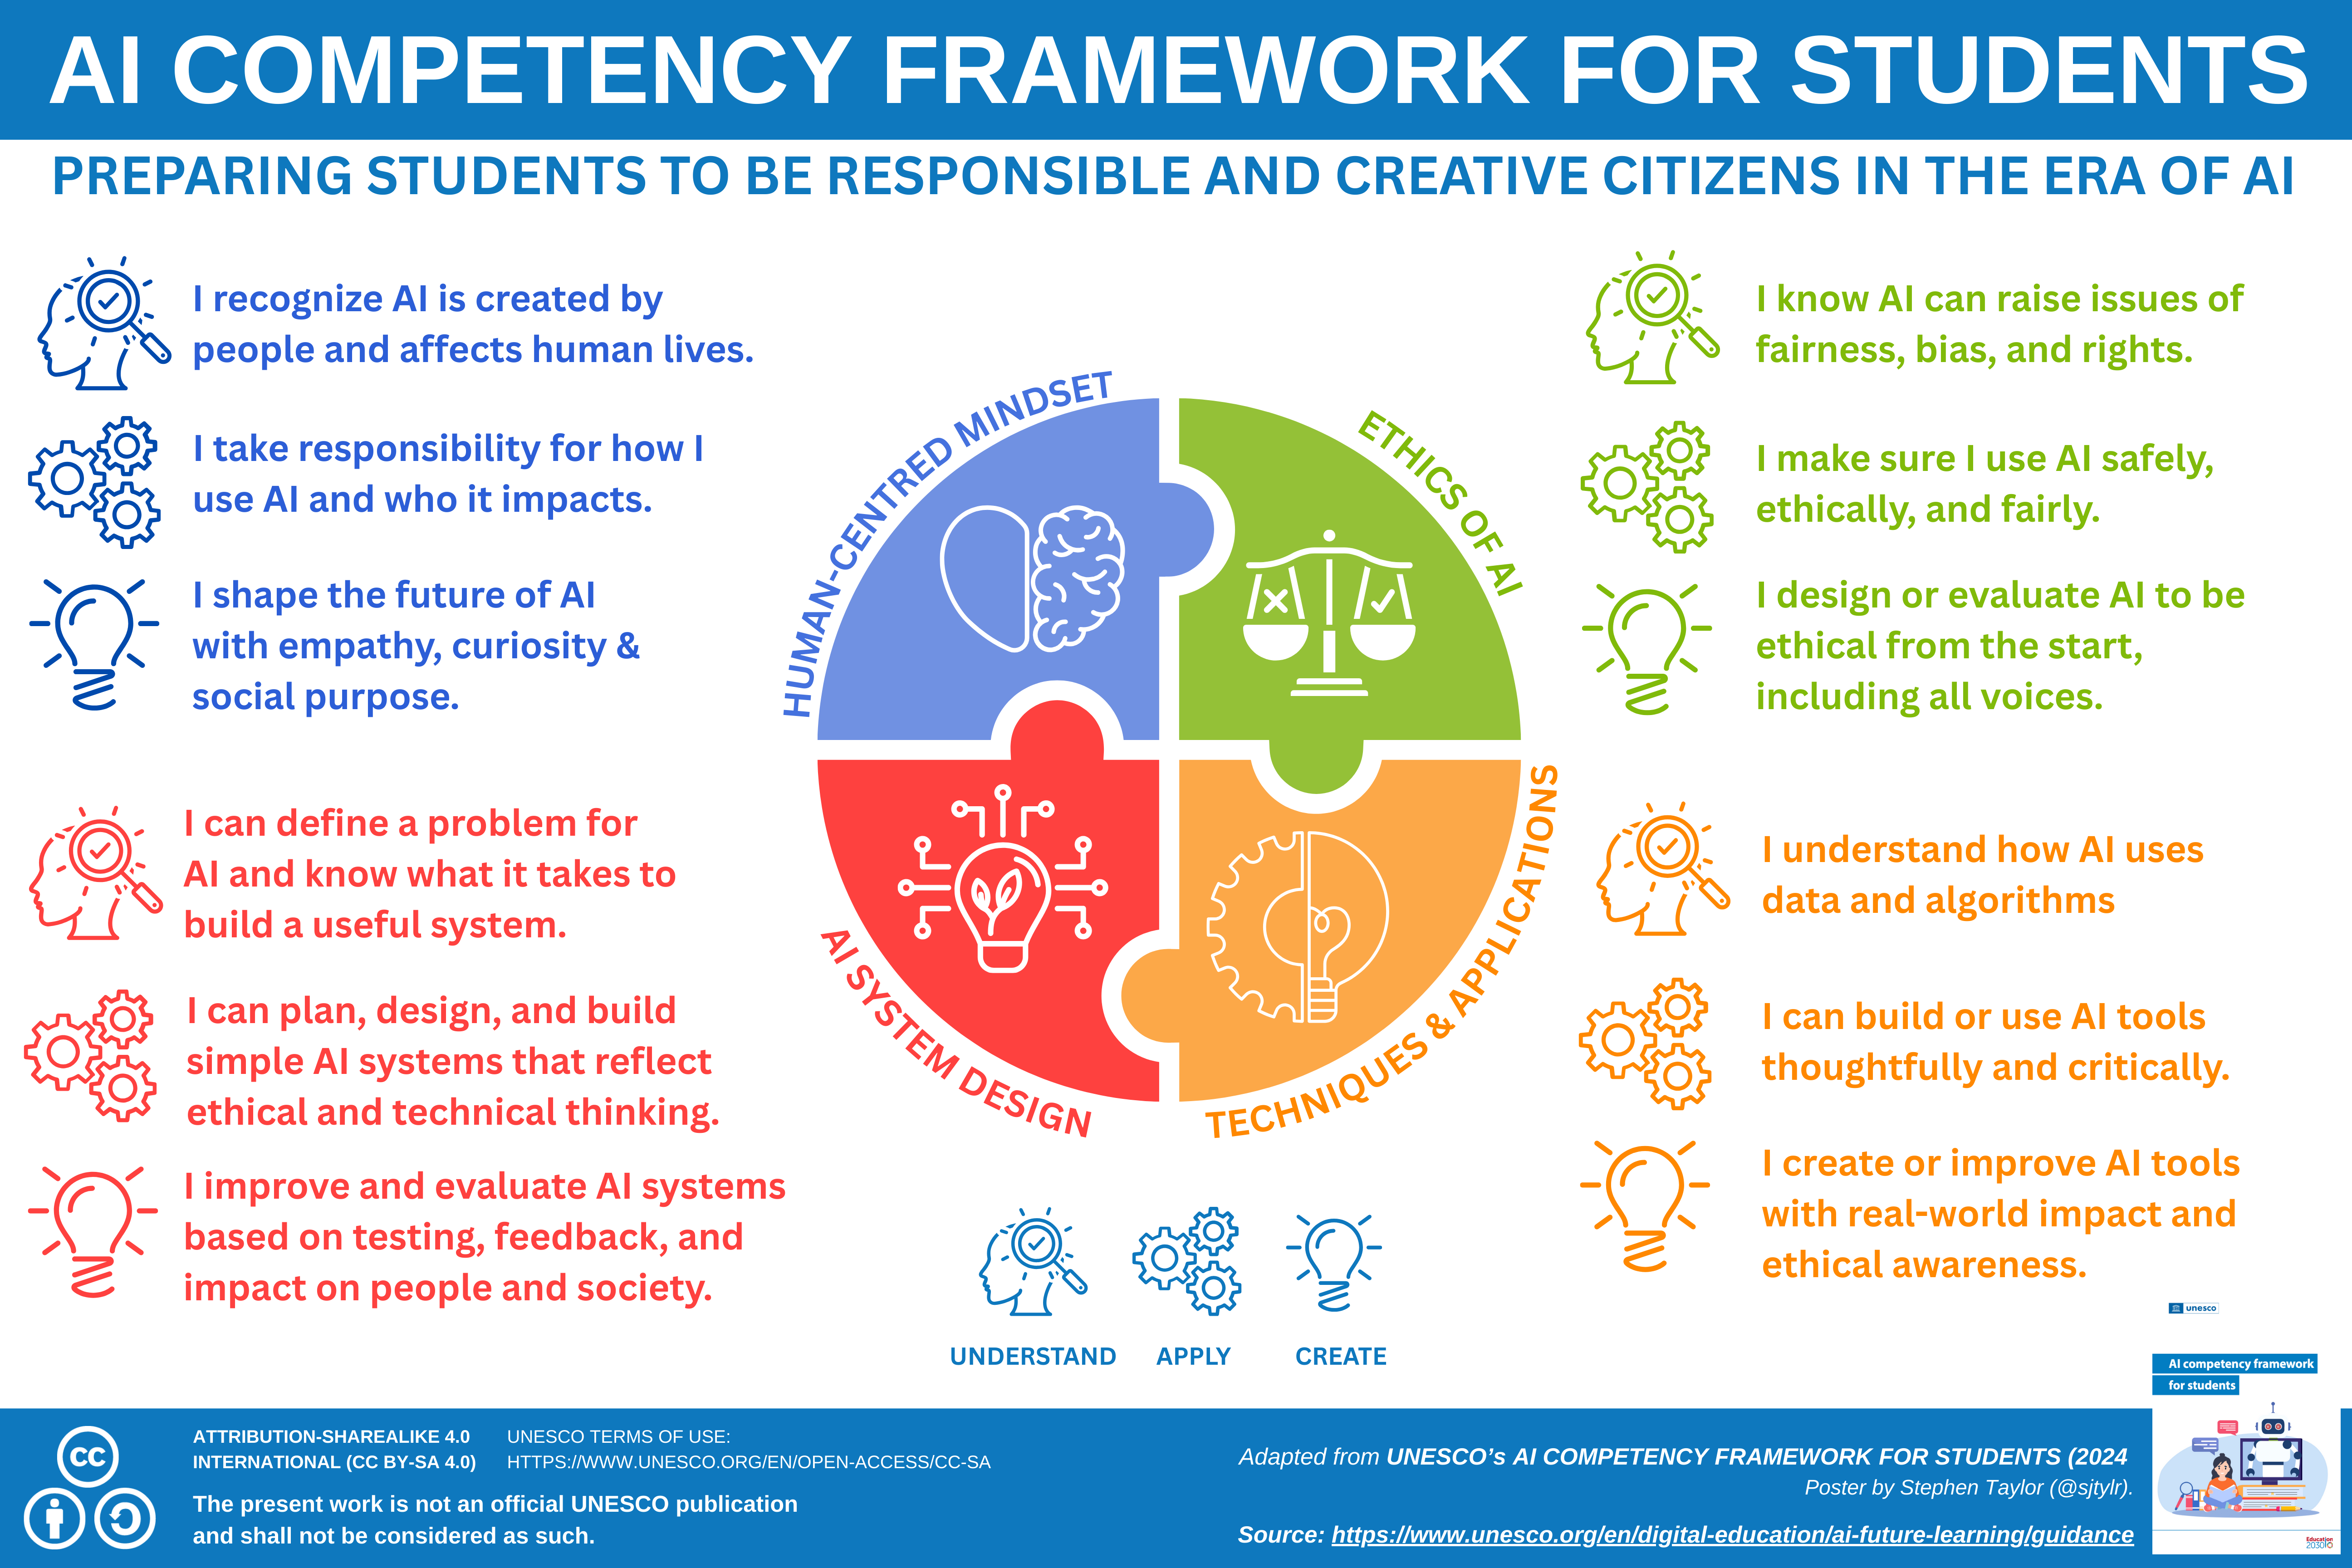
\includegraphics[scale=.1]{Chapter1/img/unesco-ai-competencies-for-students-sjtylr.png}
    \caption{Overview of UNESCO's \textit{AI Competency Framework for Students},
    which complements the teacher framework by focusing on human-centred AI, ethics, AI techniques and applications, and AI system design for responsible and creative
    student participation in the AI era. Source: adapted from the framework by
    \cite{miao2024aistudents}.}
    \label{fig:unesco-ai-competency-students}
\end{figure}

Complementing the national framework, \cite{brazil2025path} present the PATH
principles as a practical model for AI use in teaching and learning. The model draws
on international guidance, including UNESCO's AI competency frameworks for teachers
and students by \cite{miao2024aiteachers} and \cite{miao2024aistudents}.
Figure~\ref{fig:unesco-ai-competency-students} gives an overview of the student
framework, which focuses on responsible AI use, ethical awareness, basic technical
knowledge, and AI system design. The PATH principles, namely Promote teaching and
learning, Advance wellbeing and social interaction, Train for AI literacy, and
Harness AI ethically, translate these concerns into practical priorities for both
teachers and learners. They stress that AI should support teaching and learning
without replacing teacher judgement or student agency, while protecting wellbeing,
sustaining social interaction and building AI literacy within commitments to
responsibility, privacy, fairness and human rights. Read alongside the Australian
national framework, the PATH model links policy intent with classroom practice
through a human-centred approach to AI use.

Despite this relatively clear national direction, a gap remains between policy
principles and day-to-day implementation. Reports by \cite{edsafe2023aiaustralia}
and \cite{knight2023generative} describe a pragmatism gap, where schools must turn
broad ethical principles into practical action within a fast-moving and commercially
complex AI ecosystem. This helps explain why institutions such as The Hutchins
School and Virtual School Victoria have developed local policies that combine
privacy, academic integrity and teacher judgement with requirements for
transparency, consent, equity and tool review before use, as shown by
\cite{hutchins2025genai} and \cite{vsv2025aipolicy}. Recent Australian research by
\cite{lodge2023aioffloading} adds that implementation must consider AI's cognitive
effects, especially harmful cognitive offloading when students use AI to avoid the
effort required for knowledge building and critical thinking in classroom practice
contexts.

Efforts to address these challenges are reflected in local and national developments.
Although the 4E (Embrace, Enable, Experiment, and Exploit) framework by
\cite{shailendra2024framework} was proposed for university curriculum adoption, its
focus on stakeholder roles, curriculum redesign, enabling staff and students, and
evaluation offers a reference for school-level implementation. At school level, the
2024 review of the Australian framework by \cite{taskforce2025review} confirms
continuing national work on workload, data security and privacy, equity, market
power, research and copyright. Overall, Australia presents an early and well-framed
response, whose impact depends on consistent translation into classroom practice.

\subsection{United States}

The United States' approach to AI in education is characterised by a decentralised
but rapidly evolving policy landscape, where federal guidance sits alongside strong
state and local autonomy. At the federal level, the U.S. Department of Education
provides a broad ethical and policy framing for AI in teaching and learning. As set
out by \cite{usdoe2023aifuture}, it highlights possible benefits such as teacher
support, stronger adaptivity and responses to learning gaps, while warning about
bias, privacy, surveillance, inequity and the scaling of automated decisions in
education. However, implementation remains largely the responsibility of states,
districts and institutions, creating a varied and sometimes fragmented governance
landscape.

State-level initiatives play a central role in turning federal principles into
practical guidance. Washington State, for example, promotes a ``Human-AI-Human''
(H-AI-H) framework, where AI use begins with human inquiry and ends with human
reflection, insight and judgement, as set out by
\cite{washingtonospi2024implementing}. Similarly, \cite{massdese2025guidance}
provides detailed guidance that connects ethical use, equity and legal compliance
with AI literacy and teaching both with and about AI. Other states, including
Wyoming and Oregon, offer more operational guidance that links policy development
and privacy with governance, academic integrity, and responsible use, as shown by
\cite{wyomingwde2025guidance} and \cite{oregonode2023genai}. Together, these
examples show how states are translating broad AI principles into local
implementations. However, \cite{panorama2024fourstates} still suggests an uneven
landscape, where educators and district leaders continue to seek clearer and more
consistent national guidance.

At the institutional level, implementation varies across districts and educational
settings. \cite{reich2025guideai} describe the current phase as one of iterative
policy development, where schools are effectively ``building the plane while flying
it,'' favouring flexible, experimental approaches over fixed regulatory models. Some
districts gradually expand student autonomy under teacher oversight, while others
focus on teacher support and workload reduction, as shown by
\cite{northport2025guidelines} and \cite{excelsiormat2025aipolicy}.

Despite these efforts, significant concerns remain about equity and the wider social
implications of AI use in education. \cite{pennsylvaniausccr2024rising} highlights
risks related to surveillance, bias, unequal access, and the possible weakening of
teacher-student relationships if AI systems are introduced without strong
safeguards. This creates a tension between innovation-driven initiatives and the need
to protect civil rights, student privacy, and vulnerable populations. The same
concern appears in state-level toolkits and recent academic work, which stress the
importance of transparency, human oversight, teacher support, and equitable
implementation, as shown by \cite{oklahoma2025policytoolkit} and
\cite{medina2026newai}. Overall, the U.S. case shows how decentralisation can
encourage experimentation and rapid policy development, but also contributes to
fragmentation and uneven implementation across the education system, which in turn
raises concerns about equity, oversight, and the social consequences of AI in
education.

The preceding sections show how national and institutional policies define the
conditions for AI adoption in education. Yet policy documents alone cannot explain
how AI is understood, trusted, questioned or resisted by those affected by its use.
For this reason, the review now turns to public sentiment. This perspective connects
formal governance with lived educational experience, while showing where policy
ambition may diverge from stakeholder concerns, expectations and everyday practice in schools and classrooms.

\section{European Public Sentiment}
\label{c1:eps}

As mentioned in Chapter~\ref{chpt:intro}, the public sentiment component of this
study is narrower than the policy review. The policy analysis includes Ireland,
France, Australia and the United States, because looking beyond Europe can show
whether faster-moving cases offer lessons for gaps visible in European policy and
sentiment data. By contrast, directly comparable public sentiment data remains harder
to obtain across all these contexts. This section therefore focuses mainly on
European data on attitudes toward AI in education. This focus is supported by
convergence in European research, where stakeholders often show cautious optimism
about efficiency, personalised learning and innovation while raising concerns about
privacy, bias, transparency, academic integrity, human agency and the changing role
of teachers in classroom practice.

The section first reviews European-level evidence on AI and education, drawing on
studies that capture the views of young people, educators, students, school leaders,
and early adopters of GenAI in secondary education. It then briefly considers public
sentiment in Ireland and France, since these are the two European countries targeted
in this study. This structure connects three layers of evidence: European sentiment
data, national policy and public perception cases, and external policy examples that
may help interpret European policy--practice gaps. The evidence reviewed here also
shows why additional methodological support is needed later in the study. Compared
with the relatively rich set of policy documents available, sentiment material is
more uneven and less balanced across stakeholder groups and national contexts. For
this reason, these sources, together with additional documents, provide the empirical
basis for constructing an augmented textual corpus that can support a more balanced
sentiment and policy--practice analysis.

\subsection{European-level evidence}

European-level evidence suggests that public sentiment toward AI in education is
marked by cautious and conditional acceptance. Stakeholders generally recognise that
AI, especially GenAI, may support learning and feedback while reducing routine
workload and creating new opportunities for inclusion and communication. This pattern
is also visible in a recent survey by
\cite{esep2026aisurvey}, where respondents reported using AI mainly for lesson
planning and teaching materials, as well as assessment preparation, explanations,
practice exercises and administrative tasks. However, these benefits are balanced
against concerns about privacy, data use and bias, alongside misinformation,
academic integrity, pupil over-reliance, unclear guidance and the risk that automated
tools may weaken human judgement or educational relationships, as shown by
\cite{stefan2024aiyouth} and \cite{villar2025genai}.

Research on young people brings in a rights-based perspective. As shown by
\cite{stefan2024aiyouth}, young people are not only learners or users of AI systems,
but also data subjects and citizens affected by algorithmic profiling, platform
governance, and automated decision-making. From this perspective, AI literacy
includes not only technical skills but also an understanding of how AI shapes
participation, rights, well-being and democratic agency. Evidence from secondary
education shows that students and educators are already experimenting with GenAI,
often where guidance, training and support remain insufficient. Early adopters report
value in lesson preparation, feedback, summarisation and student support, while
stressing the need for teacher development, approved safe AI tools, clearer rules and
stronger ethical safeguards, as shown by \cite{villar2025genai} and
\cite{esep2026aisurvey}.

Overall, European data points to a policy--sentiment gap not in the stated values of
policy, but in their operational translation. Stakeholders often echo policy goals
around human-centred, transparent and accountable AI, yet survey results reported by
\cite{esep2026aisurvey} show that AI is already entering school practice before safe
tools, assessment rules, training and clear local guidance are fully in place. This
makes public sentiment a useful complement to policies, because it shows where
formal guidance remains too general for the practical concerns experienced by
teachers, students, youth workers and school leaders.

\subsection{National Sentiment Patterns in Ireland and France}

In Ireland, public sentiment around AI reflects the wider European pattern of
cautious optimism, where interest in innovation is tempered by concerns about trust,
regulation, transparency and long-term social impact. \cite{irfan2023irelandai} and
\cite{ucd2023aiperceptions} suggest that Irish society recognises AI's potential
across education, healthcare and industry, but acceptance remains conditional on
accountability and effective governance. These concerns are also visible in schools:
students value AI for efficiency and personalised learning but worry about critical
thinking and academic integrity, while educators recognise similar opportunities yet
report limited training, unclear guidance and uneven resources, as shown by
\cite{ai4t2023ireland}. Large-scale evidence by \cite{qqi2025genai} shows widespread
GenAI use alongside uncertainty around appropriate use, assessment and policy
clarity. Youth perspectives add a rights-based dimension, with young people seeing AI
as both an opportunity and a risk for fairness, safety and participation in
decision-making, as shown by \cite{oco2024aiyoungpeople}. Together, these findings
make the European policy--sentiment gap visible in Ireland: AI is promising, but
educational use is limited by weak guidance, uneven inclusion and support gaps.

In France, public and stakeholder sentiment around AI is visible mainly through
national surveys, European evidence, and research on digital technology use, but it
remains only partly focused on GenAI in education. Much of the evidence concerns
broader AI or digital adoption rather than classroom practice, which limits its
precision. Even so, the available sources point to a consistent pattern: AI use is
growing, but trust, guidance, and equity remain central concerns. In practice, AI
adoption among students is rising quickly. European-level data from
\cite{vodafone2025aieuschools} suggests that nearly half of French students aged
12--17 use tools such as ChatGPT, both independently and in classroom contexts,
showing growing familiarity with AI-supported learning. Students also recognise the
importance of AI skills for future careers, although regional inequalities and the
digital divide remain relevant. At societal level,
\cite{anctcredoc2025frenchaisentiment} and \cite{brice2025frenchdigitalsociety} show
increasing use of AI tools alongside caution about their role in work and everyday
life. Overall, the French case reflects a familiar European pattern: adoption is
moving faster than institutional guidance, teacher support, ethical safeguards, and
equitable access to AI competencies.

\section{NLP for Policy and Sentiment Analysis}
\label{c1:nlpsa}

The preceding sections reviewed the policy frameworks and public sentiment evidence
that shape AI in education. Together, they show that the policy--practice gap is not
located in policy documents alone, nor only in public attitudes, but in the
relationship between governance language, stakeholder concerns, and the conditions of
implementation. This section therefore turns to NLP-based and related knowledge-based
approaches that support the analysis of these relationships across policy documents,
guidance, public discourse, and stakeholder sentiment.

The section reviews six connected areas relevant to this study. First, it considers
classical text-as-data approaches, including preprocessing, document representation,
topic modelling, and methods for identifying recurring themes in large text corpora.
Second, it examines language-model-based approaches for classification, annotation,
summarisation, and discourse analysis. Third, it reviews sentiment analysis as a
distinct layer for examining how teachers, students, parents, and the wider public
express trust, concern, acceptance, or resistance toward AI use in education. Fourth,
it considers causal NLP for exploring relationships between policy language,
stakeholder sentiment, and implementation concerns. Fifth, it considers synthetic
data generation as a response to gaps, imbalance, and limited comparability in
available sentiment evidence. Finally, it briefly discusses knowledge-based
techniques, including ontologies, knowledge graphs, and GraphRAG, before explaining
why they remain outside the core scope of this study. In doing so, the section
establishes the link between the literature review and the research design developed
in Chapter~\ref{chap:method}.

\subsection{Classical Text-as-Data Approaches}

Having reviewed the policy frameworks and public sentiment evidence that shape AI in
education, the review now turns to methodological approaches for analysing policy
texts, stakeholder discourse, and public sentiment more systematically. Wider AI
governance research shows that ethical principles and high-level frameworks often
remain difficult to translate into operational processes, institutional
responsibilities, and measurable forms of implementation, as shown by
\cite{birkstedt2023ai}. In the context of AI in education, this challenge is
especially important because relevant evidence is distributed across policy
documents, institutional guidance, stakeholder discourse, public commentary, and
survey-based sentiment data.

Text-as-data methods provide a way to examine these sources at scale while retaining
a link with interpretation. Work by \cite{grimmer2013text} argues that automated
text analysis can make large-scale political and policy text collections
systematically analysable, while also stressing the need for problem-specific
validation and close interpretive judgement. Similarly, \cite{gentzkow2019text}
present text as a major source of empirical evidence for social science research,
showing how statistical and computational methods can extract structured information
from unstructured language data. Within policy research, \cite{wilkerson2017large}
show that large-scale computerised text analysis has been used to study political
communication, policy agendas, public opinion, and institutional discourse.

Topic modelling is particularly important in this tradition because it provides a
way to identify latent themes across large corpora. The original Latent Dirichlet
Allocation model by \cite{blei2003latent} remains a key reference for probabilistic
topic modelling, while structural topic models by \cite{roberts2014structural} and
\cite{roberts2016model} extend this approach by incorporating document-level
covariates, making them especially useful for comparing texts across institutions,
time periods, or policy contexts. In policy studies, \cite{isoaho2021topic}
position topic modelling as a bridge between computational analysis and qualitative
interpretation, helping researchers identify recurring themes and discursive
patterns without replacing close reading.

\subsubsection*{Preprocessing techniques}

Classical text-as-data methods depend on preprocessing because they usually
represent documents through tokens, frequencies, dictionaries, or document--term
matrices. Preprocessing therefore shapes what the model can detect and how results
are interpreted. Standard steps include removing duplicates, cleaning formatting
noise, standardising case, tokenising text, removing stop words, handling punctuation
and numbers, and deciding whether to apply stemming, lemmatisation, or phrase
detection, as outlined by \cite{welbers2017text}. These choices are not purely
technical: they can affect whether institutional terms, stakeholder categories,
negations, or domain-specific expressions remain visible in the corpus.
\cite{denny2018preprocessing} show that preprocessing decisions can substantially
affect unsupervised text-analysis results and therefore need to be tested rather than
treated as neutral defaults. Stop-word removal is particularly consequential, as
\cite{schofield2017pulling} show that it can change the interpretability and
coherence of topic-model outputs.

The importance of preprocessing is especially clear in policy and education corpora,
where sources often differ in length, formality, structure, and genre. Policy
documents may contain headings, legal phrases, bullet points, references, and
repeated institutional language, while public comments and survey responses may
contain informal wording, spelling variation, emojis, abbreviations, or short
expressions of approval and concern. In comparative and policy-oriented text
analysis, \cite{lucas2015computer} show that document preparation, translation,
metadata, and source comparability can shape downstream interpretation. For this
reason, preprocessing should be aligned with the analytical task and corpus
characteristics. Topic modelling may require careful removal of boilerplate text and
overly frequent institutional terms, while sentiment analysis requires caution
because removing negation words or intensifiers can distort the meaning of evaluative
statements. In this study, preprocessing is therefore treated as part of the research
design rather than a neutral technical step.

\subsection{Language Models for Discourse Analysis}

Recent advances in language modelling have expanded the methods available for
analysing policy texts, stakeholder discourse, and public sentiment. Earlier
text-as-data methods, such as dictionary-based analysis, classical classifiers, and
topic models, remain useful, but they often struggle with context, ambiguity,
negation, and domain-specific meaning. Smaller transformer-based models, including
BERT, RoBERTa, and DistilBERT, address some of these limits by producing contextual
representations of text, as shown by \cite{devlin2019bert}, \cite{liu2019roberta}
and \cite{sanh2019distilbert}. This makes them useful for sentiment analysis, stance
detection, document classification, and policy-topic classification, especially
where views on AI in education are mixed or conditional. Related embedding-based
approaches have also shaped topic discovery, including BERTopic, which combines
transformer embeddings with clustering and class-based TF-IDF to generate
interpretable topic representations, as proposed by \cite{grootendorst2022bertopic}.
These methods are relevant to AI-in-education governance because they support more
flexible analysis of heterogeneous sources, including policy texts, consultation
responses, survey answers, and online discourse. They also help link broad patterns
in stakeholder discourse with specific governance, implementation, and institutional
concerns.

Small Language Models (SLMs) and Large Language Models (LLMs) add a methodological
layer. Recent work by \cite{lu2024small} and \cite{nguyen2025survey} presents SLMs
as compact models designed to provide useful language capabilities with lower
computational cost, faster inference, and easier adaptation to specific tasks. This
makes them relevant for document classification, sentiment detection, weak labelling,
and policy-topic analysis, especially when the aim is to process large corpora in a
more controlled and resource-efficient way. By contrast, recent social science
research by \cite{tornberg2025llm}, \cite{heseltine2024llm} and
\cite{tornberg2024bestpractices} has explored LLMs for annotation and classification,
as well as for summarisation, qualitative coding, thematic analysis, and the
generation of synthetic or weakly labelled data. These capacities are valuable when
sources are heterogeneous, difficult to label manually, or unevenly distributed
across document types. In policy and education research, SLMs and LLMs can play
complementary roles. SLMs are useful when categories are defined and the task
requires scalable, repeatable classification across policy documents, survey answers,
or public comments. LLMs are better suited to exploratory analysis, including theme
identification, codebook refinement, initial labelling, summarisation, and
stakeholder comparison. This distinction is valuable for AI-in-education governance
because evidence is distributed across policy texts, institutional guidance, survey
evidence, and online discourse.

However, the use of language models also raises methodological concerns. SLMs depend
on suitable training or adaptation data, task-specific labels, and validation against
human-coded examples, while \cite{weber2024evaluation} and
\cite{tornberg2024bestpractices} show that LLM-based annotation requires careful
evaluation because performance can vary across models, prompts, and annotation tasks.
Recent studies by \cite{gilardi2023chatgpt}, \cite{heseltine2024llm} and
\cite{ziems2024llms} show that LLMs can perform well on text-annotation tasks,
including relevance, stance, topic, frame, sentiment, and political text
classification, but they also emphasise that model outputs should be compared with
human judgement rather than accepted uncritically. LLMs may also reproduce biases in
training data or generate fluent interpretations that appear credible without being
sufficiently grounded in the source text, making transparent prompting, source
checking, and careful reporting of model choices essential, as discussed by
\cite{bender2021stochastic} and \cite{tornberg2024bestpractices}. In policy and
sentiment analysis, language models should therefore be treated as assistive
analytical tools rather than independent sources of evidence.

\subsection{Sentiment Analysis and Stakeholder Attitudes}

Sentiment analysis provides a complementary perspective by focusing on the affective
and evaluative dimensions of text. Classic work by \cite{pang2008opinion} and
\cite{liu2012sentiment} established the field as a way to identify polarity,
subjectivity, and attitudes in textual data. More recent reviews by
\cite{tan2023survey} and \cite{mao2024sentiment} show that sentiment analysis now
includes lexicon-based, machine-learning, deep-learning, and hybrid approaches, each
with different implications for preprocessing, feature extraction, classification,
and domain adaptation. For policy and education research, this is important because
stakeholder discourse rarely expresses simple approval or rejection. Teachers,
students, parents, and the wider public may support AI-assisted learning while also
expressing concern about privacy, academic integrity, assessment, fairness, teacher
autonomy, or unequal access.

In this context, sentiment analysis should be used cautiously and in combination
with thematic interpretation. General polarity labels such as positive, negative, and
neutral may be too coarse to explain how stakeholders evaluate AI use in education.
For example, a comment may be positive about administrative efficiency but negative
about assessment integrity, or supportive of personalised learning while expressing
concern about data protection. This makes aspect-based and context-sensitive
sentiment analysis more appropriate than treating each document as having a single
overall sentiment. Work by \cite{hutto2014vader} on social-media sentiment analysis
also shows that informal language, irony, abbreviations, intensity markers, and
platform-specific expressions can affect sentiment detection, which is relevant when
analysing public comments and online discourse. In the present study, sentiment
analysis is therefore used not as a standalone measure of public opinion, but as a
way to identify patterns of trust, concern, uncertainty, and resistance that can be
compared with policy priorities and implementation challenges.

Education-focused studies illustrate this value. Recent work on GenAI in education
uses sentiment analysis alongside topic modelling to examine how public discourse
frames AI adoption, including perceived benefits, emotional reactions, and concerns
about educational consequences, as shown by \cite{so2024public},
\cite{liao2025public}, and \cite{gocen2024public}. These studies show that sentiment
analysis is most useful when it is linked to the themes, actors, and contexts being
discussed, rather than reported only as aggregate polarity. For this dissertation, the right use of sentiment analysis is therefore interpretive
and comparative: it helps reveal whether policy language around responsible,
ethical, and inclusive AI is aligned with the concerns expressed by stakeholders,
and where tensions emerge between policy ambition and public or practitioner
experience across different evidence sources, stakeholder groups, and national
contexts.

\subsection{Synthetic Data and Faithfulness Evaluation}

The analysis of public sentiment across countries and stakeholder groups is limited
by data scarcity, imbalance, and weak comparability. Available evidence often comes
from surveys, institutional reports, public comments, and academic studies that use
different sampling strategies, question formats, and levels of detail. This creates
an uneven corpus in which some countries, stakeholder groups, or sentiment positions
are better represented than others. In this context, synthetic data is used as a
controlled augmentation strategy rather than as a substitute for empirical evidence.
Its purpose is to increase the analytical coverage of under-represented categories,
support robustness testing, and make comparison between policy discourse and public
sentiment more stable. This use is consistent with \cite{argyle2023out}, which shows
that language models can approximate aggregate patterns of public opinion under
carefully specified conditions, and with wider synthetic-data research by
\cite{snoke2018general} and \cite{stanley2024synthetic}, which distinguishes between
the utility of synthetic data and its limits as a replacement for real observations.

For this study, synthetic sentiment texts are relevant because they help address
uneven evidence while keeping the analysis grounded in the original corpus and the
reviewed literature. The generated data is treated as a task-specific approximation
of stakeholder attitudes toward AI use in education, not as new empirical testimony.
It is therefore linked to documented themes such as trust, ethics, assessment,
teacher preparedness, equity, privacy, and implementation. Duplicate or
near-duplicate items are understood as texts with highly similar content after
normalisation, while irrelevant items are those with only weak relation to the study
themes. These decisions matter because they shape which forms of sentiment and
stakeholder concern remain visible in the corpus. Synthetic data is therefore used
only as a supplementary layer for exploratory and comparative analysis, with all
findings interpreted against the original empirical evidence.

The literature suggests that the faithfulness of synthetic text should be assessed
through a multi-level distance framework rather than a single similarity score.
Lexical similarity can be examined using vocabulary statistics and Jensen--Shannon
distance over word distributions, while semantic similarity can be assessed with
sentence embeddings and cosine similarity using Sentence-BERT-style representations,
as proposed by \cite{reimers2019sentence}. Distributional alignment can also be
examined in embedding space using Maximum Mean Discrepancy (MMD), a kernel-based
two-sample measure introduced by \cite{gretton2012kernel}, and Fréchet-style
embedding distance, following the broader logic of distributional evaluation in
generative modelling by \cite{heusel2017gans}. A further option is the classifier
two-sample test (C2ST) by \cite{lopez2016revisiting}, where a classifier is trained
to distinguish real from synthetic texts; performance close to chance suggests
stronger similarity, while higher accuracy indicates detectable synthetic artefacts.
In this view, faithfulness is understood in terms of usefulness rather than identity:
synthetic data is valuable only insofar as it preserves task-relevant sentiment
patterns, thematic structure, and semantic meaning while making the limits of
generated evidence explicit, following \cite{snoke2018general}.

\subsection{Causal NLP and Relational Analysis}

Causal NLP builds on a wider causal inference tradition that distinguishes causal
claims from simple associations. Foundational work by \cite{rubin1974estimating}
introduced the potential-outcomes framework for estimating treatment effects in
randomised and non-randomised studies, while \cite{pearl2009causality} developed a
structural causal modelling approach for reasoning about causal assumptions,
interventions, and confounding. These foundations matter for text-based research
because policy and sentiment corpora can reveal associations between language,
attitudes, and implementation concerns, but they do not automatically establish
causal effects. Work by \cite{egami2022causal} adapts this problem to text-as-data
research by showing how text can be used as a treatment, outcome, confounder, or
discovered measure in causal inference. Their framework is especially relevant here
because it stresses careful research design, validation of text-derived measures, and
the separation between measurement and estimation before any causal interpretation is
attempted from textual evidence and linked back to the research question.

In AI-in-education governance, causal NLP is useful because the policy--practice gap
is not only a matter of identifying themes or sentiment labels, but also of exploring
how policy priorities, stakeholder concerns, and implementation barriers may relate.
For example, policy emphasis on ethics, assessment, teacher readiness, or equity may
correspond to particular forms of public concern, institutional uncertainty, or
practical difficulty. Recent work by \cite{ma2025causal}, \cite{liu2025large}, and
\cite{wan2025large} suggests that language models can support causal relation
extraction, causal reasoning, and causal discovery from text. However, this work also
shows that these approaches remain sensitive to prompts, assumptions, data quality,
and validation. For this reason, causal NLP is best treated in this dissertation as
an exploratory and interpretive lens rather than as a basis for strong causal claims.
Its strength is that it helps move beyond isolated topics and sentiment scores toward
a more structured account of possible relationships between policy language,
stakeholder sentiment, and implementation concerns. Its weakness is that the
available evidence is observational, fragmented, and uneven across countries and
stakeholder groups, which limits causal identification and makes expert
interpretation essential.


\subsection{Knowledge-Based Alternatives}

Other computational approaches could also be used to analyse policy and education
discourse, including ontologies, knowledge bases, knowledge graphs, and Graph
Retrieval-Augmented Generation (GraphRAG). Ontologies provide explicit conceptual
structures for representing entities, relations, and categories in a domain, while
knowledge graphs organise information as interconnected nodes and edges that can
support semantic search, reasoning, and explainability. Recent work by
\cite{merono2025knowledge} demonstrates how knowledge graphs can structure rules,
responsibilities, datasets, and governance processes in more transparent and
machine-readable ways. Similarly, GraphRAG combines graph-based representations with
retrieval-augmented generation, allowing systems to retrieve not only semantically
similar text but also relational information between concepts, actors, and documents,
as discussed by \cite{peng2024graphrag}.

These approaches are promising for future work, especially where the aim is to build
a structured knowledge base of AI policy concepts, map relationships between policy
actors, or support question answering over policy documents. Tools and frameworks
such as Protégé, OWL, RDF, SPARQL, and ontology-engineering methods can support the
formal modelling of domain concepts, relationships, constraints, and inference
rules, as shown by \cite{musen2015protege} and \cite{horridge2011practical}.
However, they are not used as core methods in this study because the research
question focuses on analysing textual patterns, sentiment, and implementation
concerns rather than constructing a formal semantic representation of the policy
domain. Ontology and knowledge-graph construction would also require additional
design choices, such as schema definition, competency questions, entity linking,
relation extraction, graph validation, and query evaluation, which would
substantially expand the scope of the dissertation. For this reason, the study
prioritises NLP methods that are better aligned with its corpus-based objective:
identifying themes, sentiment patterns, and links between policy language and
stakeholder concerns.

\section*{Summary}

This chapter reviews the literature informing the study of the policy--practice gap
in AI-in-education governance. It examines how AI policy is framed, how
implementation responsibilities are discussed, and how public sentiment reveals the
conditions under which AI adoption is accepted, questioned, or resisted in
educational settings. The review treats this gap as a layered governance issue
emerging between national policy ambitions, institutional enactment, stakeholder
concerns, and the practical realities of schools and classrooms.

The chapter is organised around three connected areas. Section~\ref{c1:npf} examines
national policy and guidance documents from Ireland, France, Australia, and the
United States, comparing how different governance systems define AI-related
priorities, risks, responsibilities, and implementation expectations.
Section~\ref{c1:eps} reviews public sentiment and stakeholder perspectives, with
particular attention to European evidence as a cautious proxy for wider Western
trends. Section~\ref{c1:nlpsa} reviews computational approaches to policy and
sentiment analysis, including classical text-as-data methods, language models,
sentiment analysis, synthetic data, causal NLP, and knowledge-based techniques, as
summarised in Table~\ref{tab:nlp-policy-sentiment-methods}. Together, these areas
establish the conceptual and methodological basis for a multi-layered, data-driven
framework linking policy language, stakeholder discourse, sentiment patterns, and
implementation challenges.

\begin{table}[p]
\centering
\caption{Summary of NLP and related computational approaches in Chapter~\ref{c1:nlpsa}.}
\label{tab:nlp-policy-sentiment-methods}
\footnotesize
\renewcommand{\arraystretch}{1.25}
\begin{tabular}{
>{\raggedright\arraybackslash}p{0.16\linewidth}
>{\raggedright\arraybackslash}p{0.26\linewidth}
>{\raggedright\arraybackslash}p{0.34\linewidth}
>{\raggedright\arraybackslash}p{0.16\linewidth}
}
\toprule
\textbf{Approach} & \textbf{Main purpose} & \textbf{Relevance to this study} & \textbf{Key references} \\
\midrule

Classical text-as-data methods &
Represent documents through tokens, frequencies, dictionaries, document--term
matrices, topic models, and other structured features. &
Provide a scalable way to examine policy documents, institutional guidance, and
stakeholder discourse by identifying themes, dominant terms, discursive patterns,
and differences across countries or stakeholder groups. &
\vspace*{-.35cm}\cite{grimmer2013text, gentzkow2019text, wilkerson2017large, blei2003latent,
isoaho2021topic} \\[.15cm]

Preprocessing and corpus preparation &
Clean, normalise, tokenise, and structure textual data before modelling, including
decisions about stop words, stemming, lemmatisation, duplicates, boilerplate text,
and domain-specific terms. &
Important because preprocessing choices shape what remains visible in the corpus,
including institutional concepts, stakeholder categories, negations, intensifiers,
and AI-in-education terminology. &
\vspace*{-.35cm}\cite{welbers2017text, denny2018preprocessing, schofield2017pulling,
lucas2015computer} \\[.15cm]

Language models &
Use contextual representations, SLMs, and LLMs for classification, annotation,
summarisation, weak labelling, topic discovery, and discourse interpretation. &
Support flexible analysis of heterogeneous sources such as policy texts,
consultation material, survey answers, public comments, and online discourse. SLMs
support repeatable classification, while LLMs support exploratory coding and
interpretation. &
\vspace*{-.35cm}\cite{devlin2019bert, liu2019roberta, lu2024small, nguyen2025survey,
tornberg2025llm, ziems2024llms} \\[.15cm]

Sentiment analysis &
Identify affective and evaluative orientations in text, including polarity,
subjectivity, trust, concern, uncertainty, acceptance, and resistance. &
Helps compare stakeholder attitudes with policy priorities. It is most useful when
combined with thematic interpretation, since views on AI use in education may be
mixed, conditional, or aspect-specific. &
\vspace*{-.35cm}\cite{pang2008opinion, liu2012sentiment, hutto2014vader, tan2023survey,
mao2024sentiment} \\[.15cm]

Causal NLP and relational analysis &
Use text as a treatment, outcome, confounder, or discovered measure to explore
relationships between language, attitudes, and possible outcomes. &
Useful as an exploratory lens for examining links between policy language,
stakeholder sentiment, and implementation concerns, while avoiding strong causal
claims from uneven observational evidence. &
\vspace*{-.35cm}\cite{rubin1974estimating, pearl2009causality, egami2022causal, ma2025causal,
wan2025large} \\[.15cm]

Synthetic data and faithfulness evaluation &
Generate supplementary textual data and assess similarity to original evidence using
lexical, semantic, and distributional measures, including embedding distances and
classifier-based tests. &
Addresses data scarcity, imbalance, and weak comparability in public sentiment
evidence, but requires validation of task-relevant sentiment patterns, themes, and
semantic meaning. &
\vspace*{-.35cm}\cite{argyle2023out, snoke2018general, stanley2024synthetic,
reimers2019sentence, lopez2016revisiting} \\[.15cm]

Knowledge-based approaches &
Use ontologies, knowledge bases, knowledge graphs, and GraphRAG to represent domain
concepts, entities, relations, constraints, and links between documents or actors. &
Relevant for future work, especially for structured knowledge bases or question
answering over policy documents. They are not core methods here because the study
focuses on corpus-based analysis rather than formal semantic modelling. &
\vspace*{-.35cm}\cite{musen2015protege, horridge2011practical, merono2025knowledge,
peng2024graphrag} \\

\bottomrule
\end{tabular}
\end{table}


